\begin{landscape}
\section*{ПРИЛОЖЕНИЕ A \\ 
  (справочное) \\
  Рабочий лист Excel с результатами решения \\ базовой задачи линейного программирования}
\addcontentsline{toc}{section}{Приложение A (справочное)
  Рабочий лист Excel с результатами \\ решения базовой задачи линейного программирования}

\begin{figure}[h]
\centering
  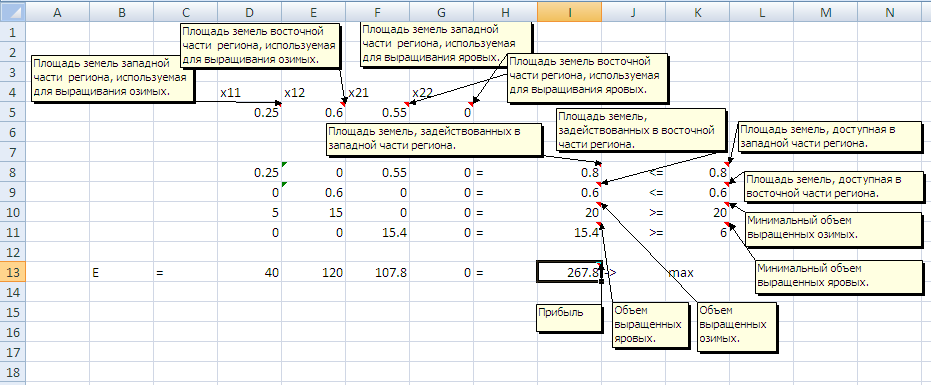
\includegraphics[width=1\linewidth]{excel}
\end{figure}

\newpage

\section*{ПРИЛОЖЕНИЕ Б \\
  (справочное) \\
  Рабочий лист Excel с результатами решения \\ модифицированной задачи линейного программирования}
\addcontentsline{toc}{section}{Приложение Б (справочное)
  Рабочий лист Excel с результатами \\ решения модифицированной задачи линейного программирования}

\begin{figure}[h]
\centering
  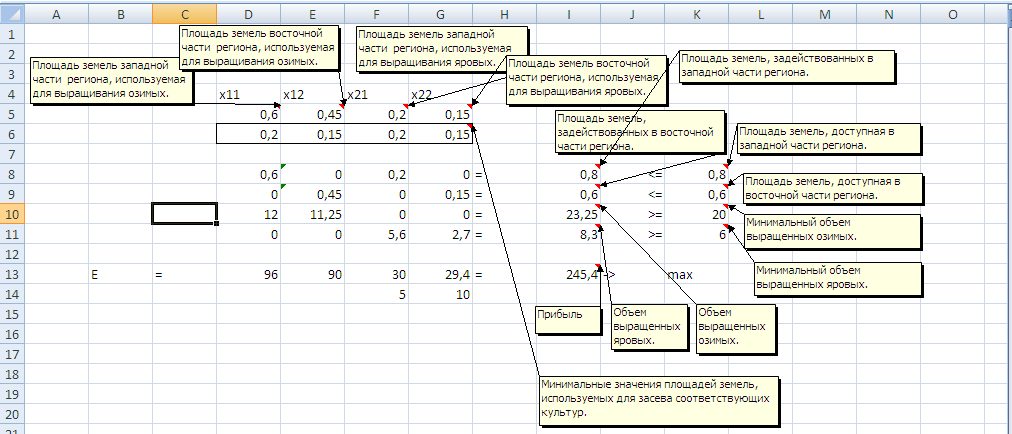
\includegraphics[width=1\linewidth]{excel_mod}
\end{figure}


\end{landscape} 